\section{Results}\label{section:Results}

A summary of all settings used for the forward and inverse calculations is presented in the appendix in tables \ref{table:settings_forw} and \ref{table:settings_inv}. In the following subsections a reasoning for these parameters will be presented and results will be shown. 

\subsection{Electrical Resistivity Tomography}
For the ERT data generation, 76 synthetic electrodes over a distance of 140 m are used to simulate the potential differences. These values are chosen as they represent a realistic field setup as it could be done as part of a thesis work. The same reasoning is also used for the other methods. Three different electrode configurations are simulated, namely the Dipole-Dipole, Schlumberger and Wenner configuration. The noise level is defined with 2.5\% and the absolute value of 0.001 mV. As the absolute noise is set very low, the data is contaminated by the relative noise magnitude. The resulting data can be visualized in terms of apparent resistivity in a pseudo section. This is shown in Figure \ref{figure:ERT_inversion_misfits} in the top row. Since no topography is considered the pseudo section directly indicates a strong subsurface anomaly as the apparent resistivities are varying between 100 $\Omega m$ and 1000 $\Omega m$. We can also see that the Dipole-Dipole configuration is generating the most data points as it shows the most cells in the section. 

Using the respective parameters in table \ref{table:settings_inv}, an inversion of the data is performed. The settings for the inversion are found by trial and assumed to be good as the data misfit value $\chi^2$ is close to 1 for all three configurations. The estimated ERT data in shown in the bottom row of Figure \ref{figure:ERT_inversion_misfits} and no significant difference between the observed and estimated pseudo sections can be observed. The resulting inverted resistivity sections are presented in Figure \ref{figure:ERT_inversion_comp}. It can be seen that all three configurations do not hold significant information below a depth of 40 m. They show a strong high-resistivity anomaly in the centre of the section at a depth between approximately 10 m and 30 m that is reaching resistivities over 10000 $\Omega m$. A shallow very conductive layer is shown up to a depth of around 10 m. Left and right of the strong resistive anomaly and below the conductive top layer another unit with resistivities of around 1000-2700 $\Omega m$ can be identified. Important to mention is that the Dipole-Dipole result appears to show slightly higher resistivity values below the conductive top layer but this is produced by the plotting. The Dipole-Dipole configuration has more measurements resulting in a higher coverage and therefore less transparent model cells. A more detailed discussion of the final inversion results of the different ERT configurations is presented in section \ref{section:Discussion}.

\begin{figure}[H]
  \centering
    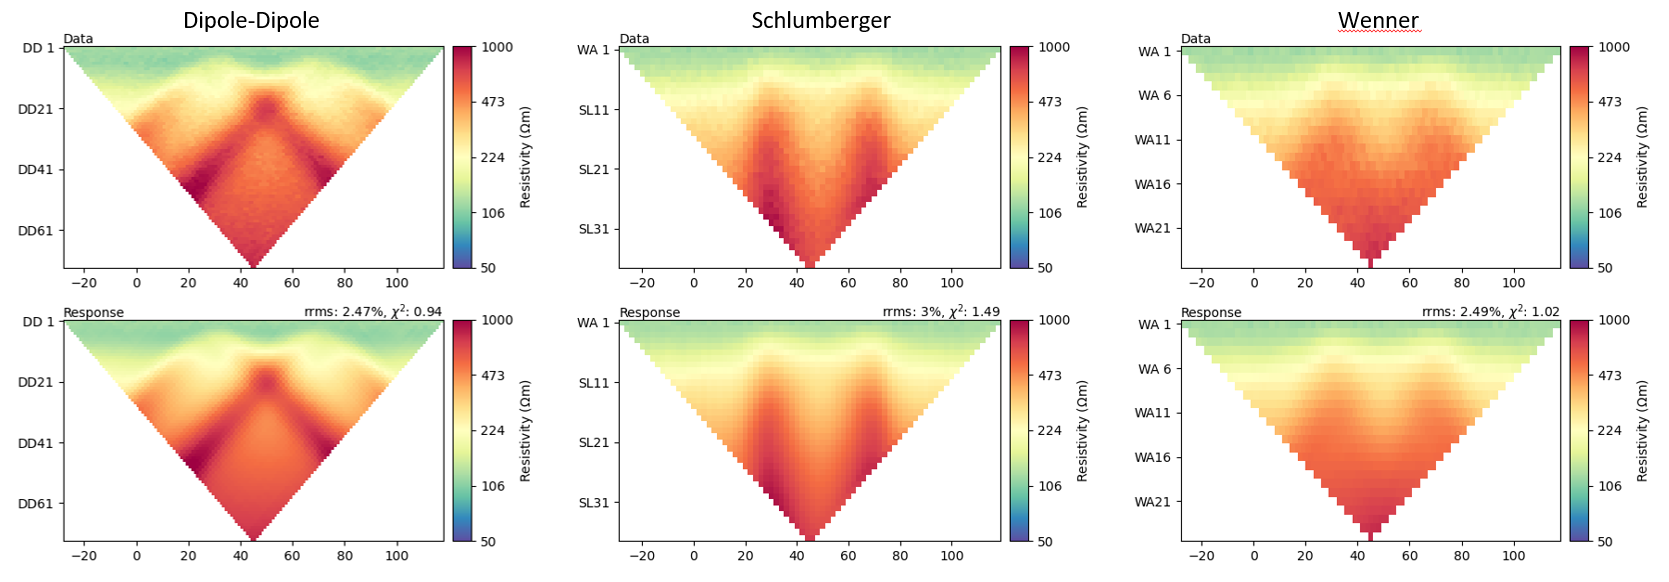
\includegraphics[width=\textwidth]{Figures/ERT_inversion_overview.png}
    \caption[ERT inversion result misfit]{Inversion result misfit of the Dipole-Dipole (left), Schlumberger (middle) and Wenner electrode configuration. At the top the synthetic data pseudo section is shown and below the pseudo section resulting from the inversion is presented. On top of the inverse model response the root mean square error (RMS) and the data misfit $\chi$ is stated.}
    \label{figure:ERT_inversion_misfits}
\end{figure}

\begin{figure}[H]
  \centering
    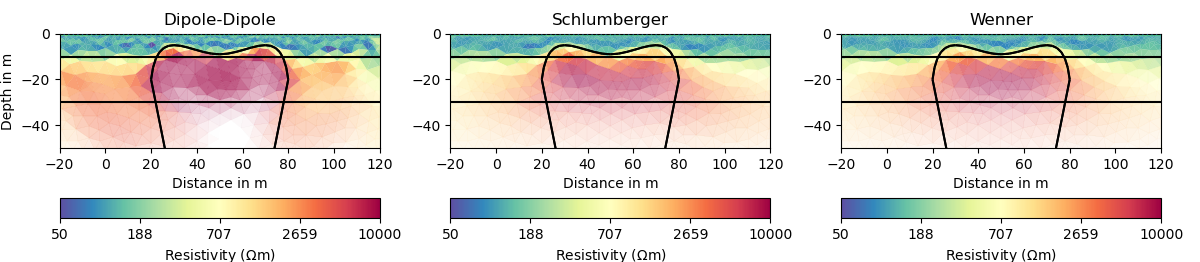
\includegraphics[width=\textwidth]{Figures/ERT_Inv_comp.png}
    \caption[Final resistivity models after inversion]{Final ERT inversion results. The results of the Dipole-Dipole (left), Schlumberger (middle) and Wenner configuration (right) are superimposed by the subsurface geometry used for synthetic data generation. The transparency of the mesh cells indicates the data coverage as opaque cells represent higher data coverage.}
    \label{figure:ERT_inversion_comp}
\end{figure}

\subsection{Seismic Refraction Tomography}\label{section:Res_TT}

For the traveltime data generation 91 sensors with a spacing of 2 m are defined between -40 m and 140 m. Every third sensor location is chosen to be a shot location, resulting in 31 shots. Just as the synthetic ERT data, noise is produced and added to the generated data. For the SRT data the absolute noise is set to 1 ms and the relative noise to 0.01 \%. This means that for early arrivals (i.e. small source-receiver offsets) the absolute noise is defining the noise magnitude while for later arrivals (i.e. large offsets) the relative noise parameter is the deciding factor. The synthetic data is presented in the left part of Figure \ref{figure:TT_inversion_misfits}. In the data matrix, the zero offset measurements (i.e. measurements with an identical source and receiver location) are excluded and appear white. The simulated traveltimes are directly converted to apparent velocities using the source receiver distance.

The inversion of the synthetic traveltimes results in an estimated data matrix which is shown in the right part of Figure \ref{figure:TT_inversion_misfits}. As seen, the data misfit is very close to one and therefore an acceptable inversion result can be assumed. Figure \ref{figure:TT_inversion_comp} presents the resulting velocity model on the left and the corresponding ray coverage on the right. As seen in the right plot, the data does not hold any information about the subsurface below 30 m depth as well as close to the left and right model boundary. Therefore, the model values in these regions are not reliable as they are not data driven but purely depending on the initial model of the iterative inversion scheme. Note that this part of the model space will not be discussed further as it does not contribute to the objectives of this synthetic data study. In the upper 10 m of the model we find a low-velocity layer which holds velocities below 1000 m/s. Between -20 m and 20 m as well as between 80 m and 120 m at a depth of 10 m to 30 m, high-velocity structures appear with velocities of 3000-3500 m/s. In between those high-velocity anomalies two velocity anomalies with around 1500 m/s (at a distance of 20-40 m and 60-80 m) appear. Between 40 m and 60 m a structure with approximately 2900 m/s can be observed. Further discussion of the results and a comparison with the other methods is presented in section \ref{section:Discussion}.

\begin{figure}[]
  \centering
    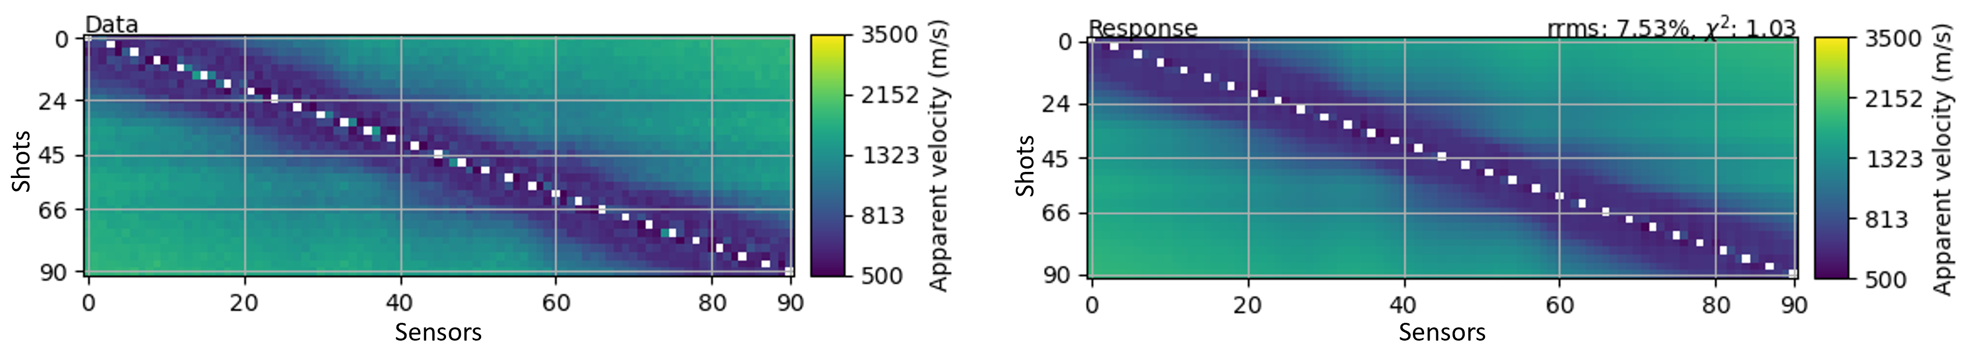
\includegraphics[width=\textwidth]{Figures/TT_RF_labels.png}
    \caption[Traveltime inversion result misfit]{Inversion result misfit of the synthetic seismic refraction tomography data. On the left, the synthetic data is shown and, on the right, the estimated data resulting from the inversion is presented. On top of the inverse model response, the root mean square error (RMS) and the data misfit $\chi$ is stated.}
    \label{figure:TT_inversion_misfits}
\end{figure}

\subsection{Gravimetry}
According to table \ref{table:settings_forw} the synthetic gravity data was generated using a 140 m long spread of 71 stations. As no inversion is performed on this synthetic data set, no noise is generated and superimposed on the data. The synthetic gravity measurements can be seen in Figure \ref{figure:grav}. As the parameter table \ref{table:properties} states, the diatreme has a lower density than the surrounding dense sandstone and therefore produces a negative gravity response in the synthetic data. Due to the irregular upper boundary of the diatreme structure two saddle points in the gravity anomaly can be observed at 30 m and 70 m. Figure \ref{figure:grav} also shows that the anomaly reaches its maximum magnitude of approximately -0.3 mGal at a distance of 50 m which coincides with the center axis of the diatreme structure.

\begin{figure}[H]
  \centering
    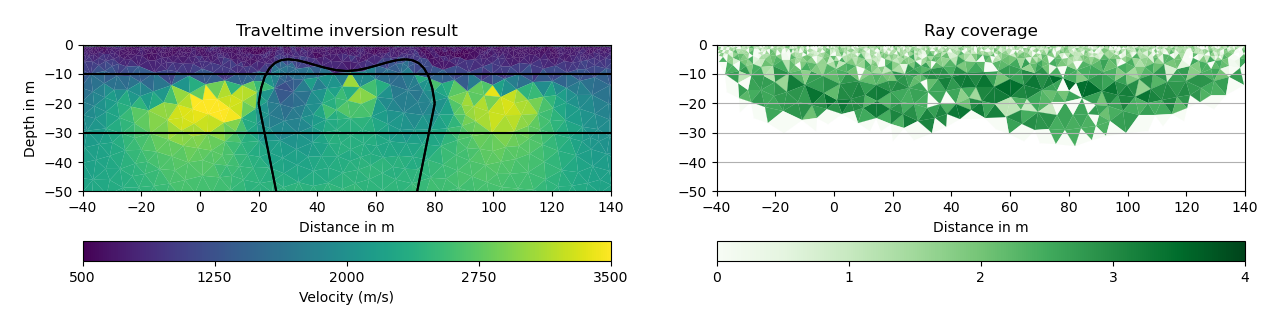
\includegraphics[width=\textwidth]{Figures/TT_comp.png}
    \caption[Final velocity model after inversion]{Final traveltime inversion results. The final velocity model (left) is superimposed by the subsurface geometry used for synthetic data generation. The ray coverage of the SRT is shown on the right.}
    \label{figure:TT_inversion_comp}
\end{figure}
\begin{figure}[H]
  \centering
  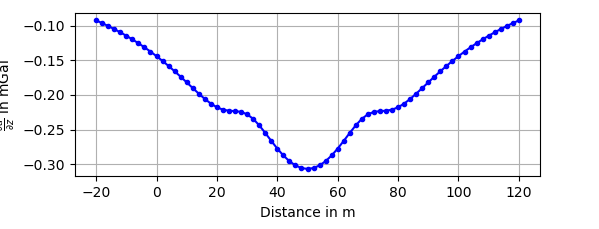
\includegraphics[width=0.8\textwidth]{Figures/GRVA_dataonly.png}
    \caption[Synthetic gravity data]{Synthetic gravity data points.}
    \label{figure:grav}
\end{figure}


